\section{Uvod}
Računalna moć uređaja koje gotovo neprestano nosimo sa sobom, kao što su pametni telefoni i prijenosna računala unazad deset godina eksponencijalno je narasla. 
Naravno, s modernim alatima dolaze i moderni problemi. 

Jedan od najraširenijih alata koji se danas koristi za rješavanje algoritamski nemogućih ili izrazito kompliciranih problema je \emph{umjetna inteligencija}.
Umjetna inteligencija podrazumjeva skup načina i metoda koje računalu opisuju početno i konačno stanje do kojeg mora doći sam.

Ovaj rad će se baviti najkorištenijom metodom umjetne inteligencije, \emph{dubokim učenjem}, i njegovim podskupom \emph{računalnim vidom}.
Kroz rad i programsku implementaciju prihvatiti ću se problema detekcije napisanog teksta na slici i daljnom obradom istog. \\
Detaljno ću kroz poglavlja obraditi postupke koje sam primjenio za generiranje raznolikih slika koje imitiraju rukopis i proces potreban da računalo nauči prepoznavati isti na slici.

Na kraju izlučeni tekst sa slike, biti će moguće obraditi na željeni način.
Način koji ću predstaviti biti će primjena jednostavne matematike, slično onome što pruža \emph{Photomath, Inc.}. 
Na primjer, za sliku na kojoj je napisan tekst \texttt{"2 + 2"}, izlaz će biti slika sa kvadratima oko prepoznatih simbola, i rješenje obrađenog teksta, u ovom slučaju \texttt{"4"}.

\section{Računalni vid}

\subsection{Pregled}
Na najvišoj razini, \emph{računalni vid} su metode koje koje računalima daju mogućnost razumjevanja slike na visokoj razini, najčešće s ciljem automatiziranja ljudskih poslova.
Osnovni zadatak je raspoznavanje veze između obrazaca na slici i rješenja problema koji se želi riješiti. 
Svi procesi koji koriste strojno učenje u konačnici se svode na  detekciju i klasifikaciju elemenata na slici.
Metode računalnog vida temelje se na geometriji, statistici, fizici i teoriji učenja. \\
Danas se velika količina problema rješava uz pomoć računalnog vida, često da ljudi toga nisu ni svjesni:
\begin{itemize}
\item Prepoznavanje znakova (Slika ~\ref{fig:cv_traffic_1})	
\item Prepoznavanje lica
\item Kompresija i restauracija slike
\item Prepoznavanje elemenata na slici
\item Analiza medicinskih snimki u svrhu detaljnije analize
\item Itd.
\end{itemize} 

\begin{figure}[h!]
	\centering
	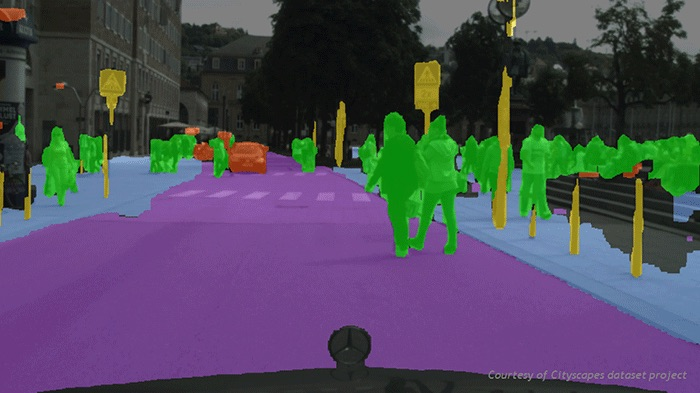
\includegraphics[width=0.8\linewidth]{cv_traffic}
	 \caption{Maskiranje elemenata na slici prometa}
 	 \label{fig:cv_traffic_1}
\end{figure}

\subsection{Konvolucijske neuronske mreže}
Konvolucijske neuronske mreže su podskup dubokih neuronskih mreža, većinom primjenjene nad vizualnom mediju (slika, video) \cite{ConvNet}.
Glavna prednost nad potpuno povezanim neuronskim mrežama je manji broj \emph{težina} za učenje što ga i cijeli proces znatno ubrzava. 
Ipak, ono što je možda najvažnije za napomenuti je to što pozicija traženog elementa na slici \emph{konvolucijskoj neuronskoj mreži} ne igra ulogu. 

Svaki sloj \emph{duboke konvolucijske neuronske mreže} funkcionira kao filter koji se kreće po slici, pamteći što ga je najviše aktiviralo. Najčešće se koristi filter veličine $3\times3$.
(Slika ~\ref{fig:conv_net_1})

Dalje, uz konvolucijski sloj, nerijetko se postavlja \emph{max pooling sloj}.
Na apstraktnoj razini, princip rada max pooling sloja je sljedeći: Ako uzmemo veličinu pooling filtra kao onu koja se najčešće koristi, to jest $2\times2$, on izlaz iz prethodnog sloja raspodjeli na kvadrate iste veličine. Zatim, filter se postavi između 4 kvadrata i sebi za vrijednost stavi najveću iz svakog u pripadajuće polje. \\ 
Prirodno je pitati se zašto se to koristi i zašto to radi. \\
Pooling filter jednostavno smanjuje "rezoluciju" prethodnog sloja, ne mjenjajući važne čimbenike potrebne za daljnji rad mreže. 
Na primjer, vertikalna linija, krug, ili elipsa, ostaje ono što jest jedino manje razlučivo. 
Bitno je napomenuti da smanjivanjem rezolucije dobivamo puno manje parametara za učenje. 
Stavimo to u brojeve. \\
Slike unutar \emph{mnist} seta podataka su veličine $28\times28$.
To znači da bi se učilo $28*28$ parametara. 
Primjenom \emph{Max pooling sloja} veličine $2\times2$, učilo bi se $\frac{1}{4}\times(28\times28)$ parametara. 

\begin{figure}[h!]
	\centering
	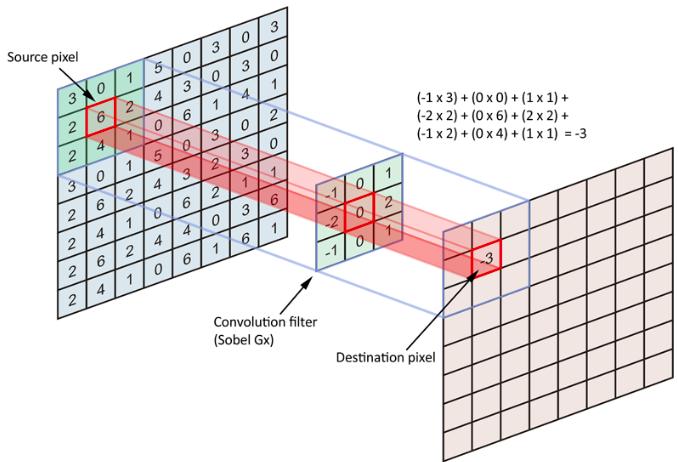
\includegraphics[width=0.8\linewidth]{conv_net}
	 \caption{Klizeći konvolucijski filter}
 	 \label{fig:conv_net_1}
\end{figure}

Spomenute prednosti referenciraju se na glavnu značajku \emph{konvolucijskih mreža}. 
Cilj je ići dublje, ne šire. 
Za sliku veličine $100\times100$, potpuno povezanoj neuronskoj mreži u prvom sloju treba \texttt{10 000} čvorova, svaki sa svojim parametrom za treniranje, dok konvolucijskoj to ne treba. \\
Svaki sljedeći sloj ima drugu ulogu. 
Prvi najčešće ima ulogu raspoznavanja najosnovnijih elemenata slike kao što su različiti rubovi, dok sve dublji koriste podatke od prošlih i osnovne elemente grupiraju u apstraktne strukture koji predstavljaju značajnije elemente slike (\cite{o2015introduction}).
